
$\quad\;\:$В данном разделе будет рассмотрен модельный эксперимент с использованием регуляризаторов в BigARTM. Его задачей является демонстрация использования реализованного механизма регуляризаторов, от него не ожидается получения ответов на какие-либо исследовательские вопросы.

\subsection{Описание эксперимента} 
$\quad\;\:$Производится обучение двух тематических моделей --- с регуляризатором и без. Для регуляризации модели используется регуляризатор сглаживания/разреживания (в данном эксперименте будем использовать только разреживание). Параметры эксперимента следующие:

\begin{enumerate}
	\item Обучающая коллекция документов --- NIPS ($\approx$ 1600 документов).
	\item Объём словаря --- $\approx$ 13000 терминов.
	\item Число внешних итераций --- 12, внутренних --- 5.
	\item Число процессоров --- 2.
	\item Число тем --- 16
\end{enumerate} 

Регуляризация имеет следующую траекторию:
\begin{itemize}
	\item 0 --- 2 итерации: нет регуляризации;
	\item 3 --- 4 итерации: на каждой внешней итерации от счётчиков $n_{wt}$ отнимается 15;
	\item 5 --- 6 итерации: на каждой внешней итерации от счётчиков $n_{wt}$ отнимается 25;
	\item 7 --- 8 итерации:  на каждой внешней итерации от счётчиков $n_{wt}$ отнимается 40;
	\item 9 --- 11 итерации: на каждой внешней итерации от счётчиков $n_{wt}$ отнимается 60;
\end{itemize}

\subsection{Результаты эксперимента}

\begin{figure}[h!]\center
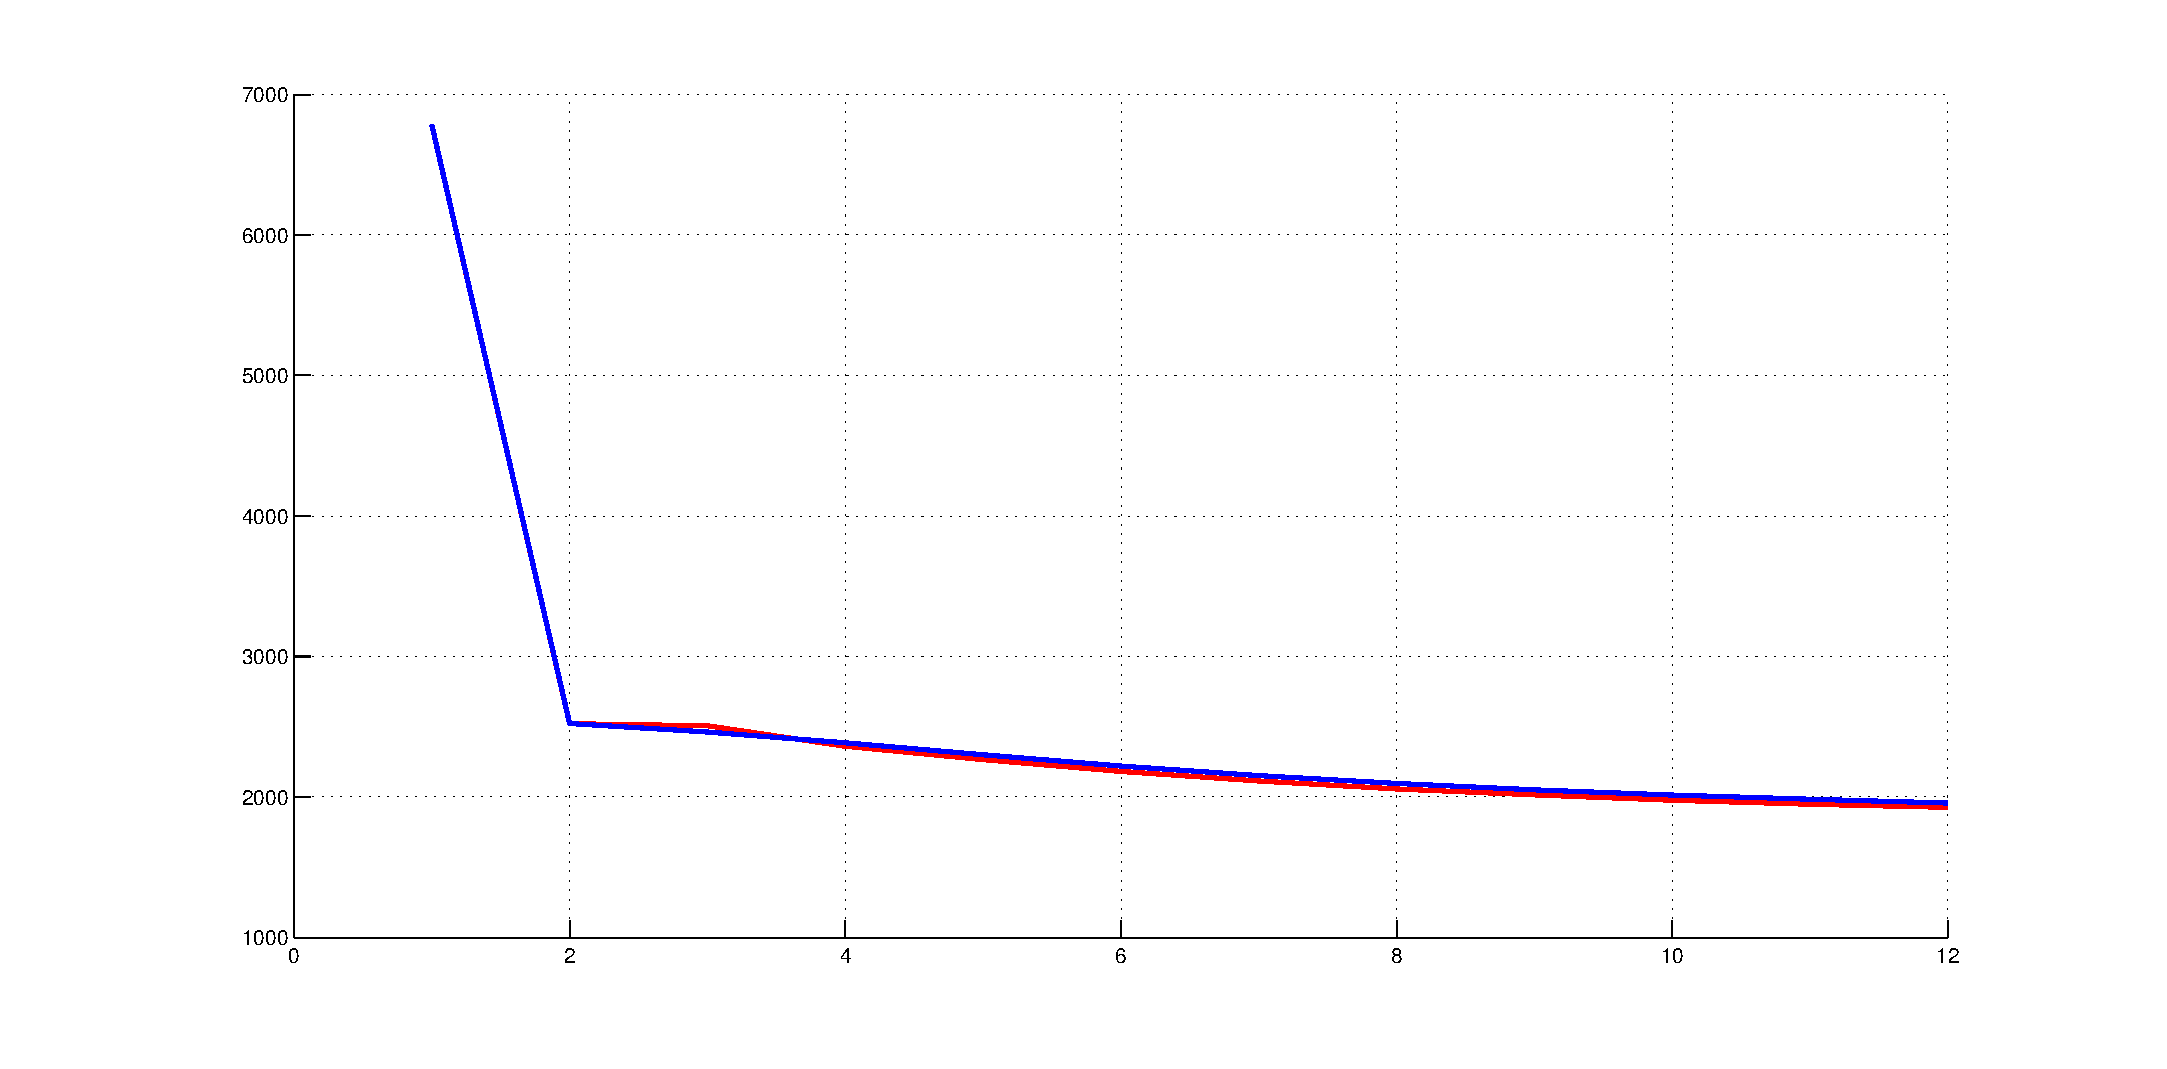
\includegraphics[scale = 0.5]{perplexity.eps}
\caption{Ось X --- номер внешней итерации, ось Y --- перплексия модели на обучающей выборке. Красная линия соответствует регуляризованной модели, синяя --- нерегуляризованной}
\label{pic_1}
\end{figure}

$\quad\;\:$Значимыми параметрами качества тематической модели являются различность тем, разреженность матриц $\Phi$ и $\Theta$ (без учёта фоновых тем), объём ядер тем (т.е. слов, характеризующих данную тему). Регуляризация имеет перед собой задачу оптимизировать именно эти величины, не ухудшив при этом переплексию по сравнению с нерегуляризованной моделью. В BigARTM на данный момент отсутствует механизм оценивания параметров матрицы $\Theta$, поэтому ограничимся одним критерием --- степенью разреженности матрицы $\Phi$. Как видно из графиков на \ref{pic_1}, регуляризация модели не изменила существенно перплексию на обучающей выборке. В то же время, разреженность матрицы $\Phi$ существенно повысилась, что очевидно из графиков на \ref{pic_2}.

\begin{figure}[h!]\center
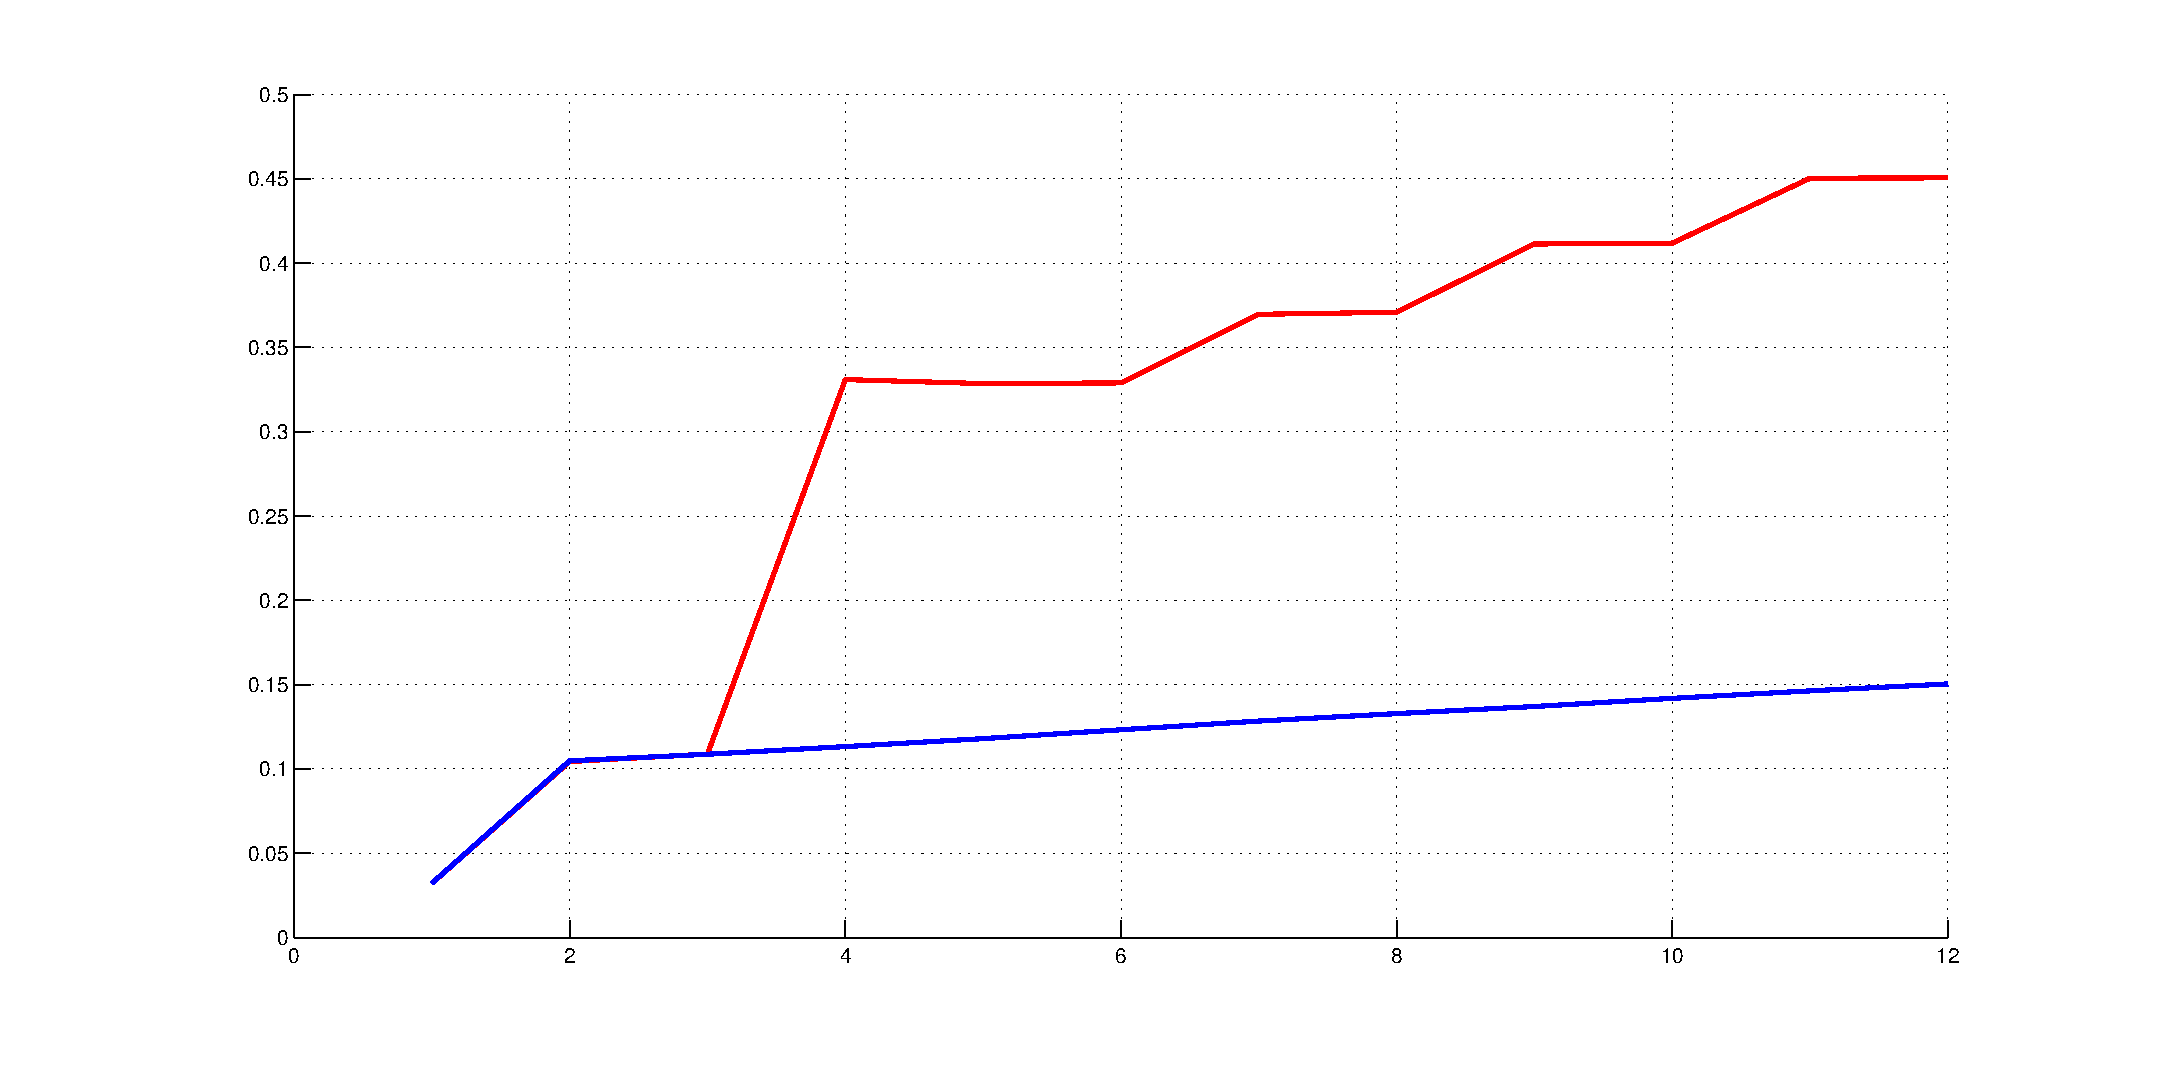
\includegraphics[scale = 0.5]{sparsity.eps}
\caption{Ось X --- номер внешней итерации, ось Y --- разреженность матрицы $\Phi$ в процентах от общего числа элементов. Красная линия соответствует регуляризованной модели, синяя --- нерегуляризованной}
\label{pic_2}
\end{figure}